\chapter{Chosen gestures}
\label{chap:chosen-gestures}

This chapter introduces the gestures that this project aims to recognize. The establishement of a ground truth is discussed in section \ref{sec:wizard-of-oz-experiment} and the selected gestures for this project presented in section \ref{sec:gestures}.

\section{Wizard of Oz experiment}
\label{sec:wizard-of-oz-experiment}

In collaboration with Caroline Biewer and Thomas Holdener writing a master thesis in psychology \cite{psychology} a setup was designed, where probands of a Wizard of Oz experiment would sit in front of a beamer screen and control an application (Google Earth and Powerpoint) through gestures (see figure \ref{fig:survey}). In this setup the probands were recorded in stereo according to the environmental constraints established in section \ref{sub:environmental-constraints} and wearing two gloves of the first version. This study had the goal of analyzing movements with regard to the comprehensiveness, comfort and learnability of their use in a usability evaluation. For this, the illusion of a working gesture recognition system was created, where in fact the "wizard of oz" was directly controlling the application with the keyboard and the mouse. The ergonomic gestures project helped provide this illusion by positioning two PS3 cameras in front of the probands and let them wear the color-marked gloves.

The stereoscopic recordings were intended to be used as a ground truth as well as to determine wich types of gestures were preferred for controlling a visual application. Unfortunately, due to unfavorable lighting conditions and several redesigns of the glove, the recordings were incompatible with later versions of the Ergonomic Gestures Recognition architecture.
\begin{figure}[H]
   \centering
   \subfloat{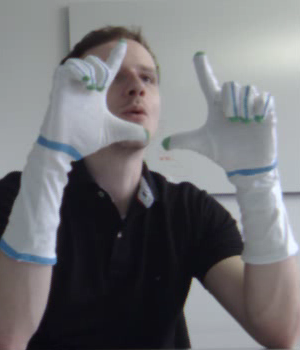
\includegraphics[width=0.235\textwidth]{images/survey1}}
      \hspace{0.01\textwidth}
   \subfloat{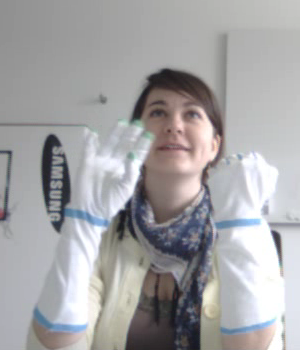
\includegraphics[width=0.235\textwidth]{images/survey2}}
      \hspace{0.01\textwidth}
   \subfloat{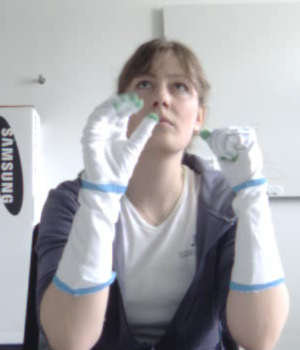
\includegraphics[width=0.235\textwidth]{images/survey3}}
      \hspace{0.01\textwidth}
   \subfloat{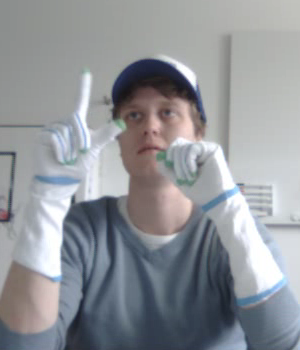
\includegraphics[width=0.235\textwidth]{images/survey4}}
   \caption{Participants performing gestures}
   \label{fig:survey}
\end{figure}

\section{Gestures}
\label{sec:gestures}

After several glove redesigns and the use of monocular videos instead of stereoscopic videos, this project focused to recognize the following gestures, performed by the right hand:
\begin{itemize}
\item Pointing gesture: Index finger pointing upwards, other fingers contracted but with visible markers
\item Zooming gesture: Index an thumb finger pointing upwards, zoom line between index and thumb more horizontal than vertical
\item Horizontal swiping gesture: swiping motion mostly carried out by wrist, not the whole arm.
\end{itemize}

\begin{figure}[H]
	\centering
	\subfloat[Pointing]{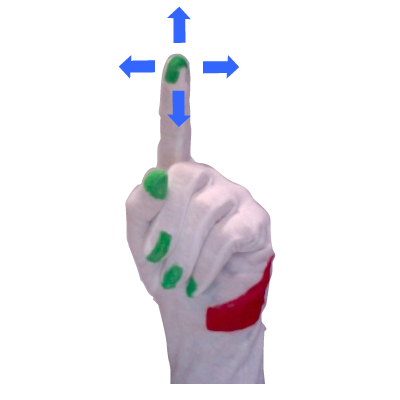
\includegraphics[width=0.22\textwidth]{images/gesture_pointing}}
	\hspace{0.03\textwidth}
	\subfloat[Zooming]{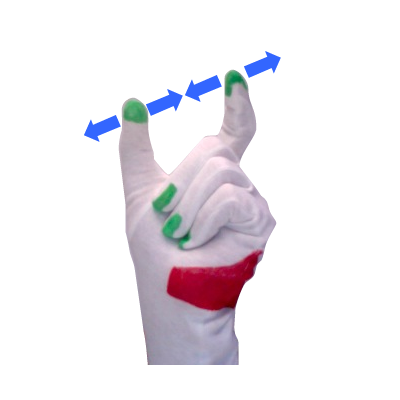
\includegraphics[width=0.22\textwidth]{images/gesture_zooming}}
	\hspace{0.03\textwidth}
	\subfloat[Swiping]{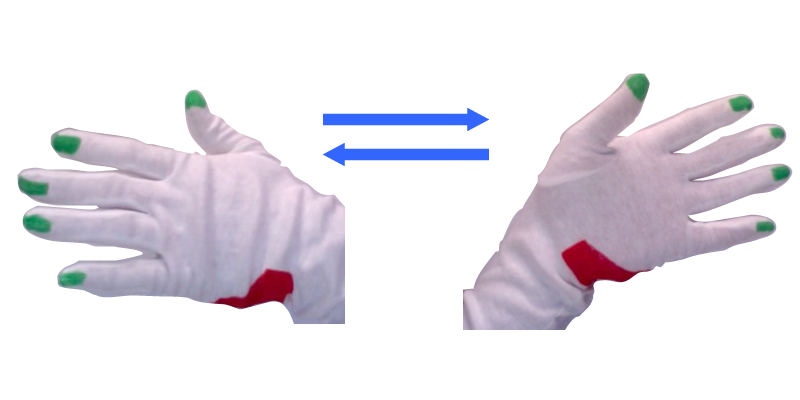
\includegraphics[width=0.44\textwidth]{images/gesture_swiping}}
	
	\caption{Gestures with motions labeled as arrows}
	\label{fig:gestures}
\end{figure}

These gestures were recorded in different videos containing all three gestures with no particular order and containing a single type of gesture repeated several times. In each video the gestures were performed exactly according to the specifications, but while trying maximize the wrist position variability.
